\section{Evaluation}\label{evaluation}
\begin{figure}
	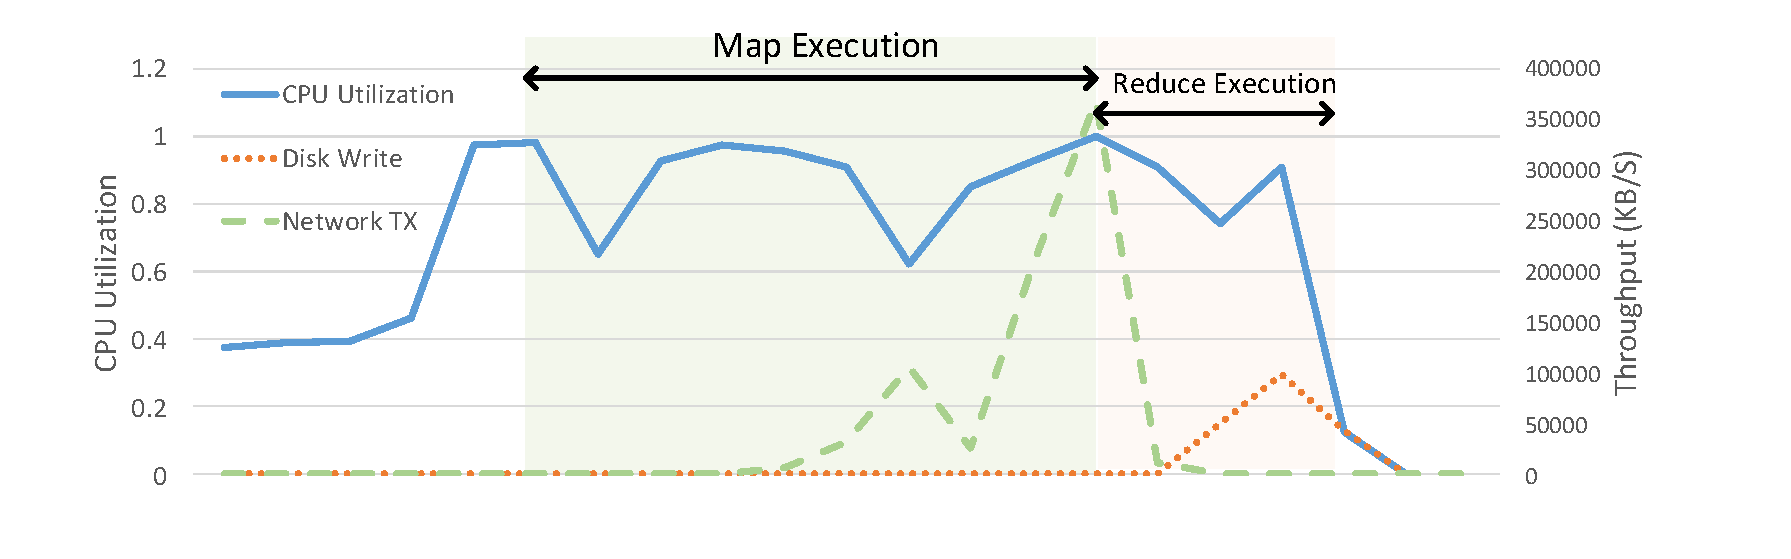
\includegraphics[width=\linewidth]{fig/scache_util}
	\caption{CPU utilization and I/O throughput of a node during a Spark single shuffle application With SCache}
	\label{fig:scache_util}
\end{figure}
In this section, we present the evaluation results of Spark with SCache comparing with the original Spark.
We first run simple DAG computing jobs with two stages to analyze the impact of shuffle optimization.
In addition, we run a shuffle heavy benchmark named Spark Terasort \cite{spark-tera} to evaluate the SCache under different inputs with different partition schemes.
In order to prove the performance gain of SCache with a real production workload, we also evaluate Spark TPC-DS \cite{sparktpcds} and present the overall performance comparison.
At last, we evaluate the overhead of weighted reservoir sampling. Because a complex Spark application consists of multiple stages. The completion time of each stage varies under different input data, configurations and different number of stages. This uncertainty leads to the dilemma that dramatic fluctuation occurs in overall performance comparison. To present a straightforward illustration, we limit the scope of most evaluations in a single stage.
\subsection{Setup}\label{stepup}
We run our experiments on a 50 m4.xlarge nodes cluster on Amazon EC2 \cite{aws}. Each node has 16GB memory and 4 CPUs. The network bandwidth is not specifically provided by Amazon. Our evaluations reveal the bandwidth is about 300 Mbps (see Figure \ref{fig:util}).

\subsection{Simple DAG Analysis}
\subsubsection{Hardware Utilization}
We first run the same single shuffle test (GroupByTest from Spark example \cite{sparksource}) as mentioned in Figure \ref{fig:util}. As shown in Figure \ref{fig:scache_util}, the hardware utilization is captured from one node during the job. Note that since the completion time of whole job is about $50\%$ less than Spark without SCache, the duration of Figure \ref{fig:scache_util} is cut in half as well. An overlap between CPU, disk and network can be easily observed in Figure \ref{fig:scache_util}. That is, the I/O operations will never cut off the computing process with the fine-grained resource allocation. By running Spark with SCache, the overall CPU utilization of the cluster stays in a high level. The decoupling of shuffle write from map tasks frees the CPU earlier, which leads to a faster map task computation. The shuffle pre-fetch starts the shuffle data transfer in the early stage of map phase shift the network transfer completion time, so that the computation of reduce can start immediately after scheduled. And this is the main performance gain we achieved on the scope of hardware utilization by SCache.
\begin{figure}
	\begin{subfigure}{\linewidth}
		\centering
		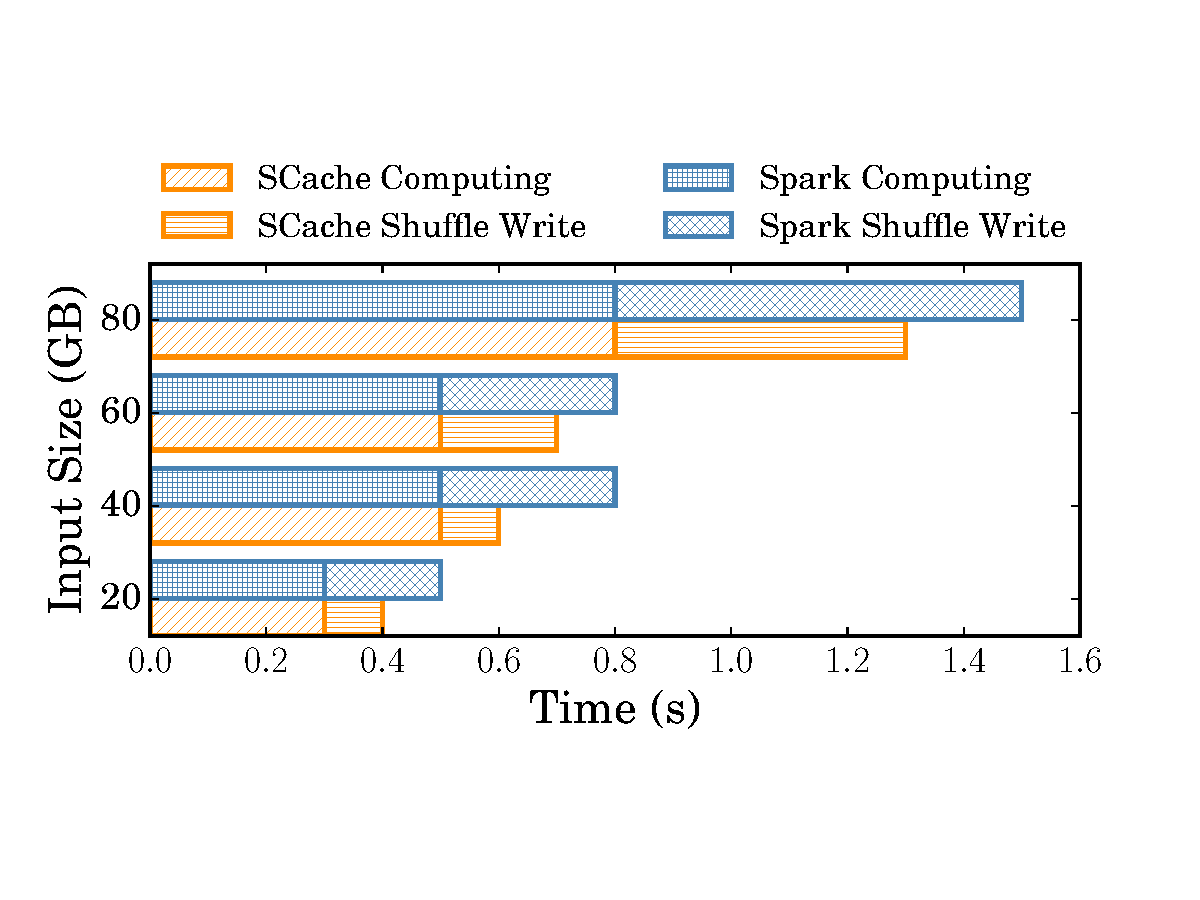
\includegraphics[width=0.9\linewidth]{fig/groupbymaptask}
		\caption{Median Task Details in Map Stages}
		\label{fig:maptask}
	\end{subfigure}
	\begin{subfigure}{\linewidth}
		\centering
		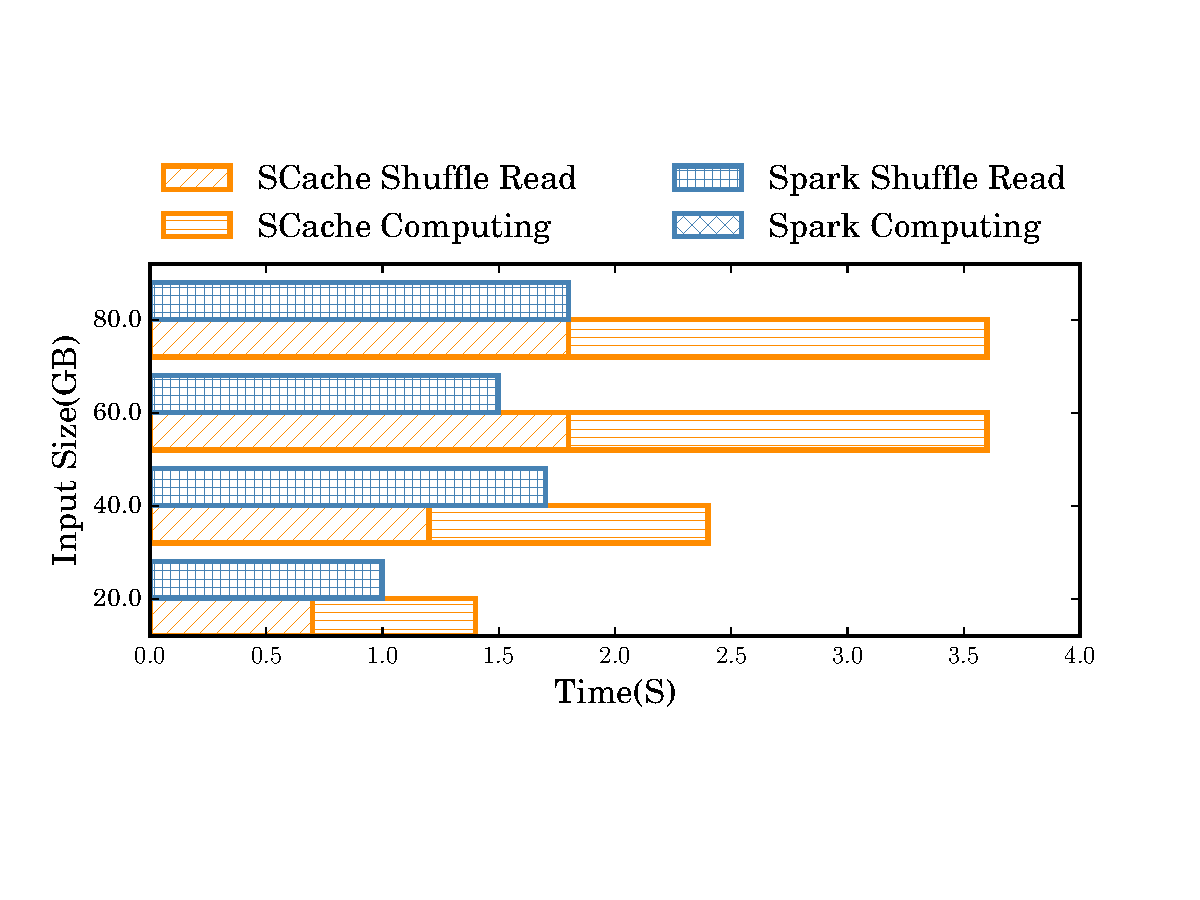
\includegraphics[width=0.9\linewidth]{fig/groupbyreducetask}
		\caption{Median Task Details in Reduce Stages}
		\label{fig:reducetask}
	\end{subfigure}
	\caption{Median Task Completion Time of Single Shuffle Test}
	\label{fig:singleshuffletask}
\end{figure}

As shown in Figure \ref{fig:singleshuffle}, we run the single shuffle test with different input sizes in the cluster. For each stage, we run 5 rounds of tasks. The stage completion time is presented separately in Figure \ref{fig:mapstage} and Figure \ref{fig:reducestage}. By running spark with SCache, the completion time of map stage can be reduced $10\%$ on average. For reduce stage, instead, SCache achieves a ~$75\%$ performance gain in the completion time of the reduce stage.

A detail analysis into the nutshell of varied overall performance gain on different stages is presented with Figure \ref{fig:singleshuffletask}. For each stage, we pick the median task. About 40\% of shuffle write time can be eliminated by SCache (Figure \ref{fig:maptask}) in a map task. Because the serialization of data is CPU intensive \cite{makingsense} and it is inevitable while moving data out of Java heap memory, SCache can not eliminate the whole phase of shuffle write. This results in a less performance gain in the map stage.
On the reduce side, the network transfer introduces a significantly latency in shuffle read for a single task (Figure \ref{fig:reducetask}). By doing shuffle data pre-fetch for the reduce tasks in Figure \ref{fig:reducetask}, the shuffle read time decreases ~$100\%$, which means shuffle data pre-fetch almost hide all the explicit network transfer in the reduce stage. In overall, SCache can help Spark decreases by ~$89\%$ time in the whole shuffle process. In addition, heuristic reduce tasks scheduling achieves better load balance in cluster than the Spark default FIFO scheduling which may randomly assign two heavy tasks on a single node. So that we can have a significant performance gain in the completion time of the reduce stage.
% \begin{figure*}
% 	\begin{minipage}{\textwidth}
% 		\begin{figure}[H]
% 			\begin{subfigure}{0.5\textwidth}
% 				\centering
% 				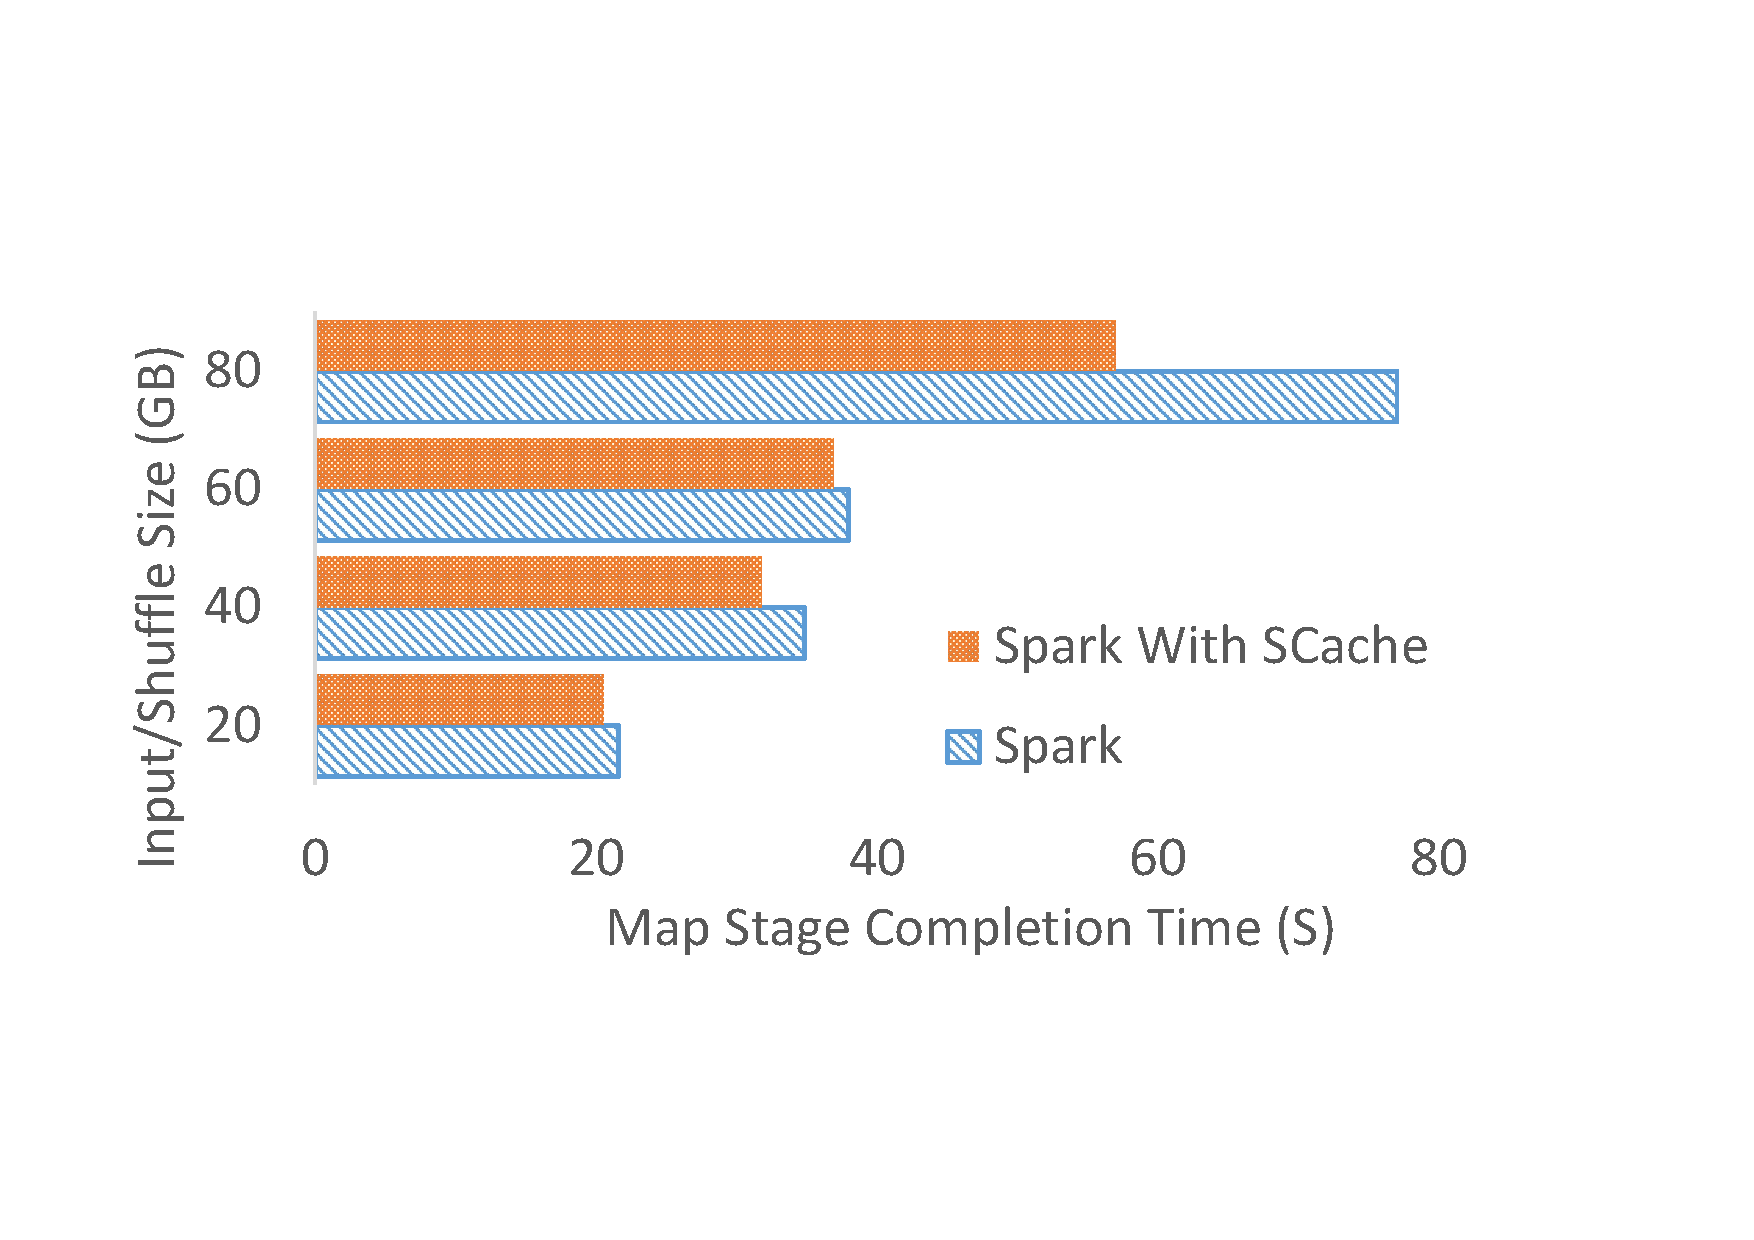
\includegraphics[width=0.8\linewidth]{fig/groupbymapstage}
% 				\caption{Map Stage Completion Time Comparsion}
% 				\label{fig:mapstage}
% 			\end{subfigure}
% 			\begin{subfigure}{0.5\textwidth}
% 				\centering
% 				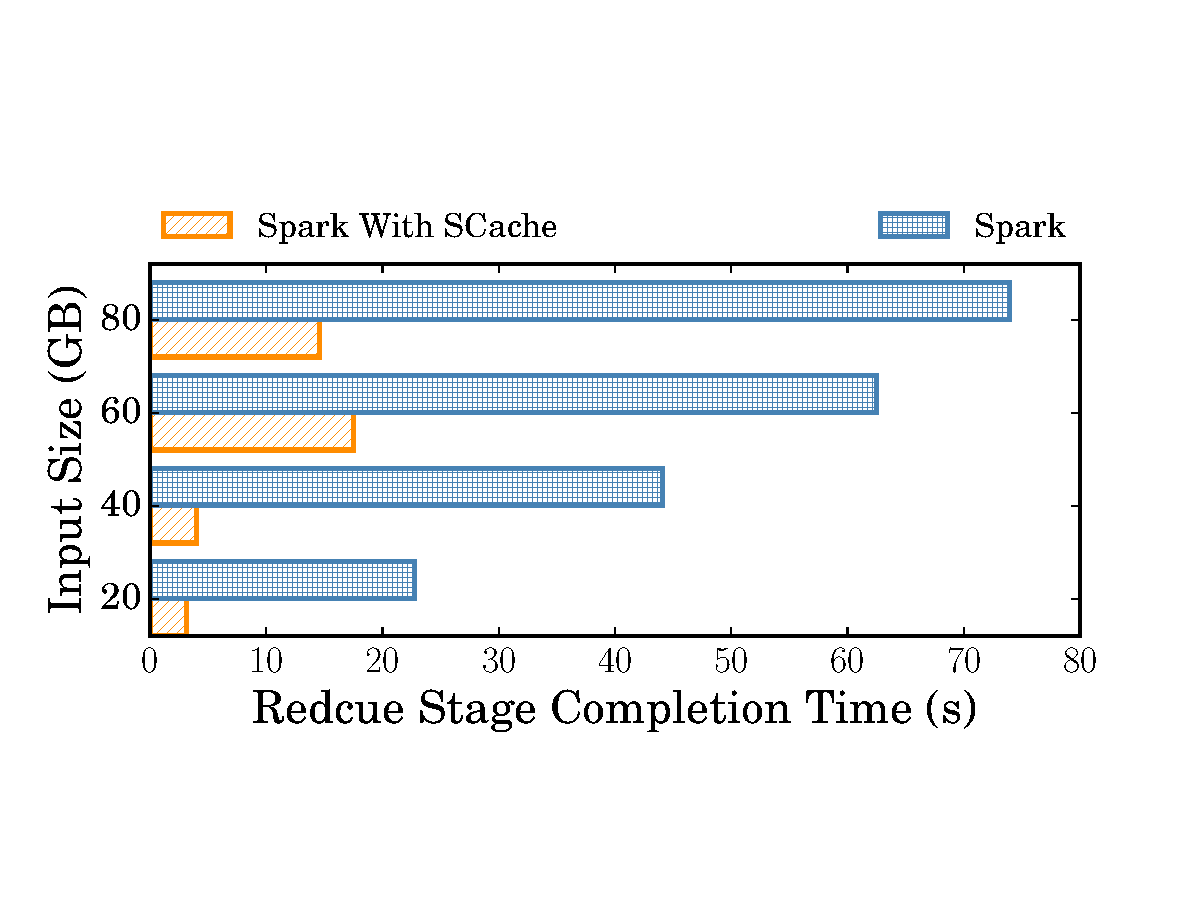
\includegraphics[width=0.8\linewidth]{fig/groupbyreducestage}
% 				\caption{Reduce Stage Completion Time Comparsion}
% 				\label{fig:reducestage}
% 			\end{subfigure}
% 			\caption{Stage Completion Time Comparsion of Single Shuffle Test}
% 			\label{fig:singleshuffle}
% 		\end{figure}
% 	\end{minipage}
% 	\begin{minipage}{\textwidth}
% 		\begin{figure}[H]
% 			\begin{subfigure}{0.5\textwidth}
% 				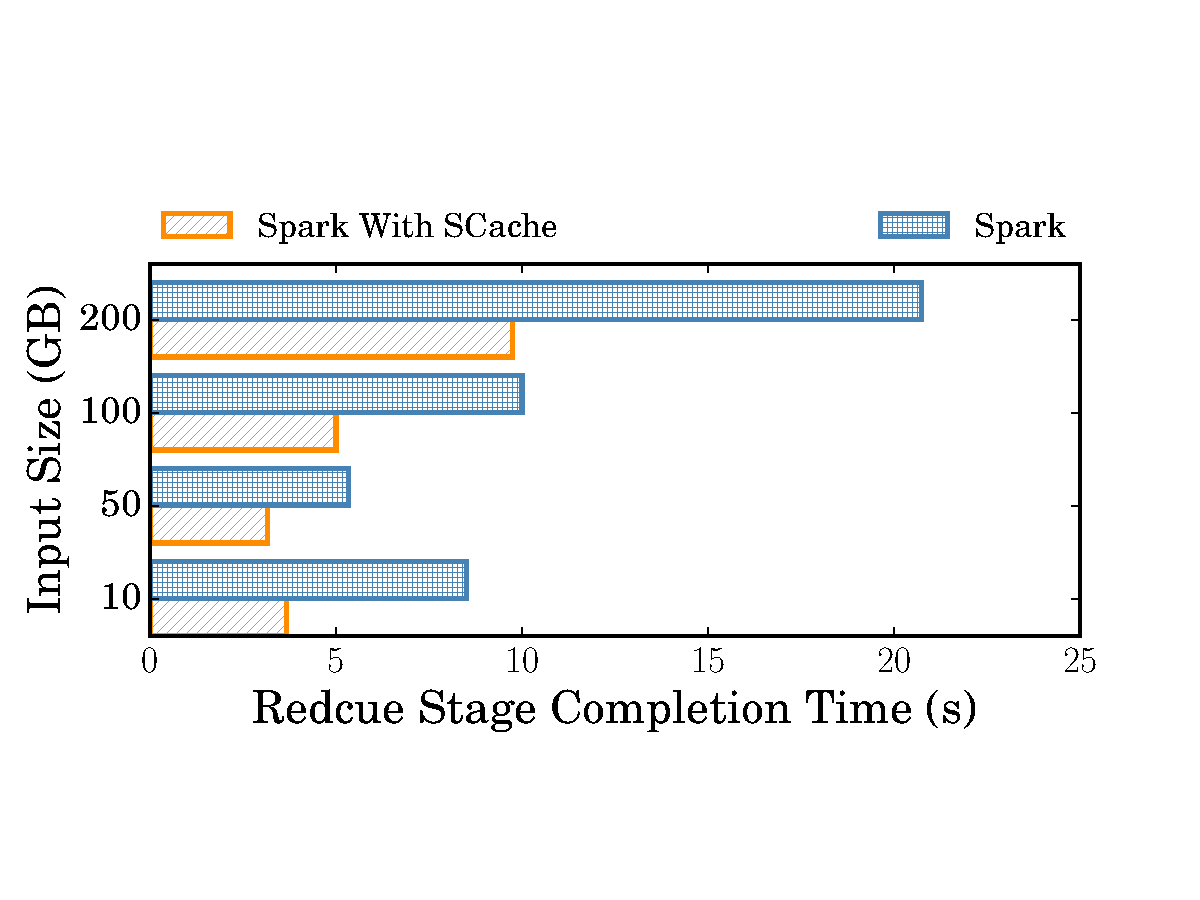
\includegraphics[width=0.8\linewidth]{fig/tera}
% 				\caption{Reduce Stage Completion Time Comparsion}
% 				\label{fig:terasort}
% 			\end{subfigure}
% 			\begin{subfigure}{0.5\textwidth}
% 				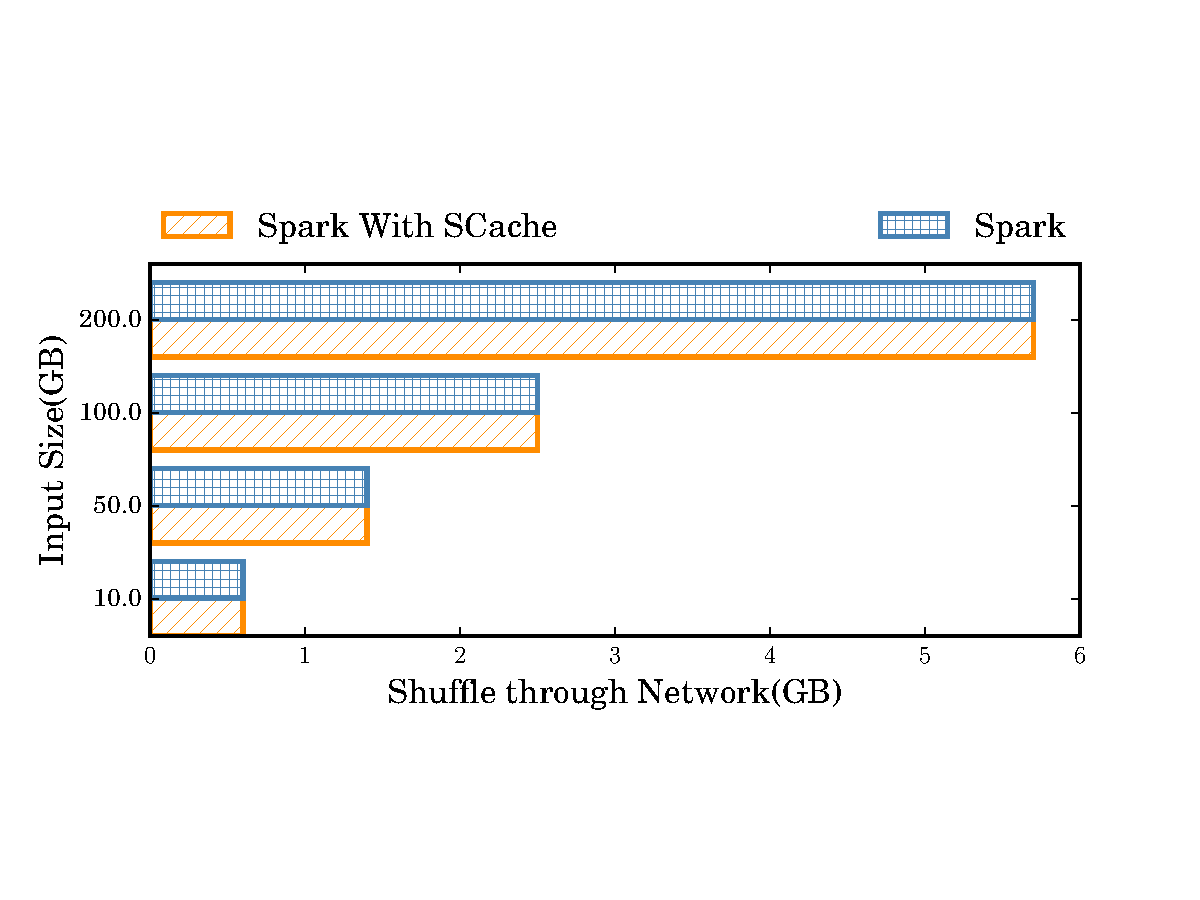
\includegraphics[width=0.8\linewidth]{fig/tera_shuffle}
% 				\caption{Shuffle Data Size Comparsion}
% 				\label{fig:terashuffle}
% 			\end{subfigure}
% 			\caption{Terasort Evaluation}
% 		\end{figure}
		
% 	\end{minipage}
%  \end{figure*}
\begin{figure}
	%\vspace*{-0.01cm}
	\begin{subfigure}{\linewidth}
		\centering
		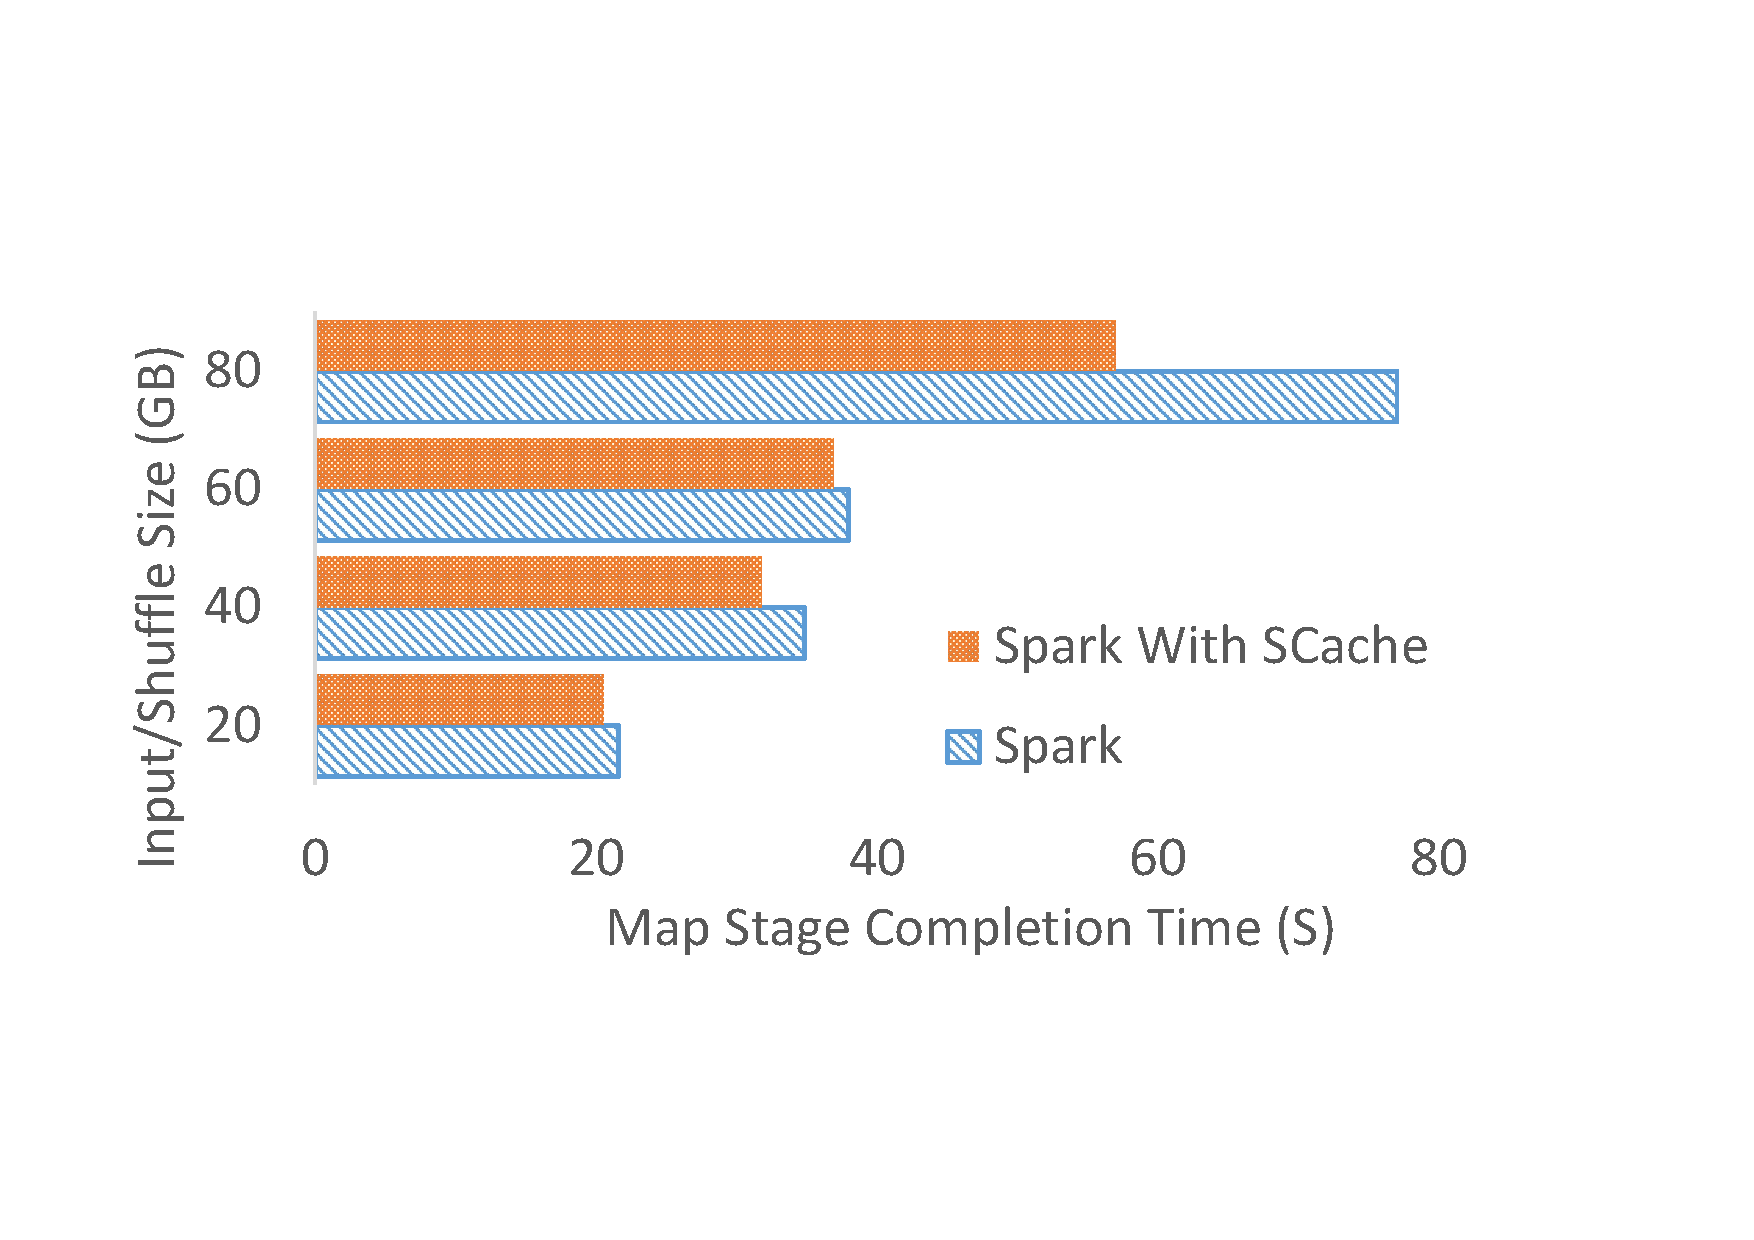
\includegraphics[width=0.9\linewidth]{fig/groupbymapstage}
		\caption{Map Stage Completion Time Comparison}
		\label{fig:mapstage}
	\end{subfigure}
	\begin{subfigure}{\linewidth}
		\centering
		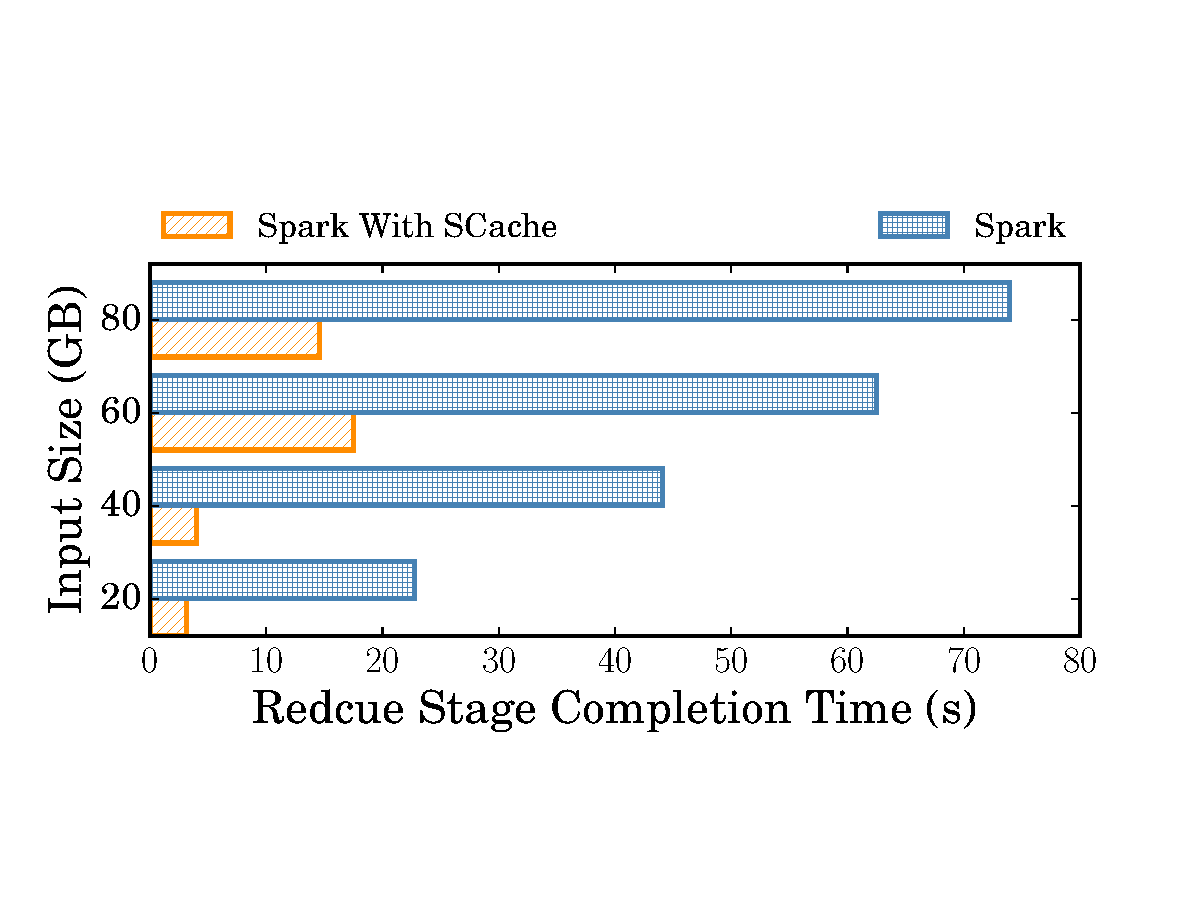
\includegraphics[width=0.9\linewidth]{fig/groupbyreducestage}
		\caption{Reduce Stage Completion Time Comparison}
		\label{fig:reducestage}
	\end{subfigure}
	\caption{Stage Completion Time of Single Shuffle Test}
	\label{fig:singleshuffle}
\end{figure}
% \begin{figure}
% \begin{subfigure}{\linewidth}
% 	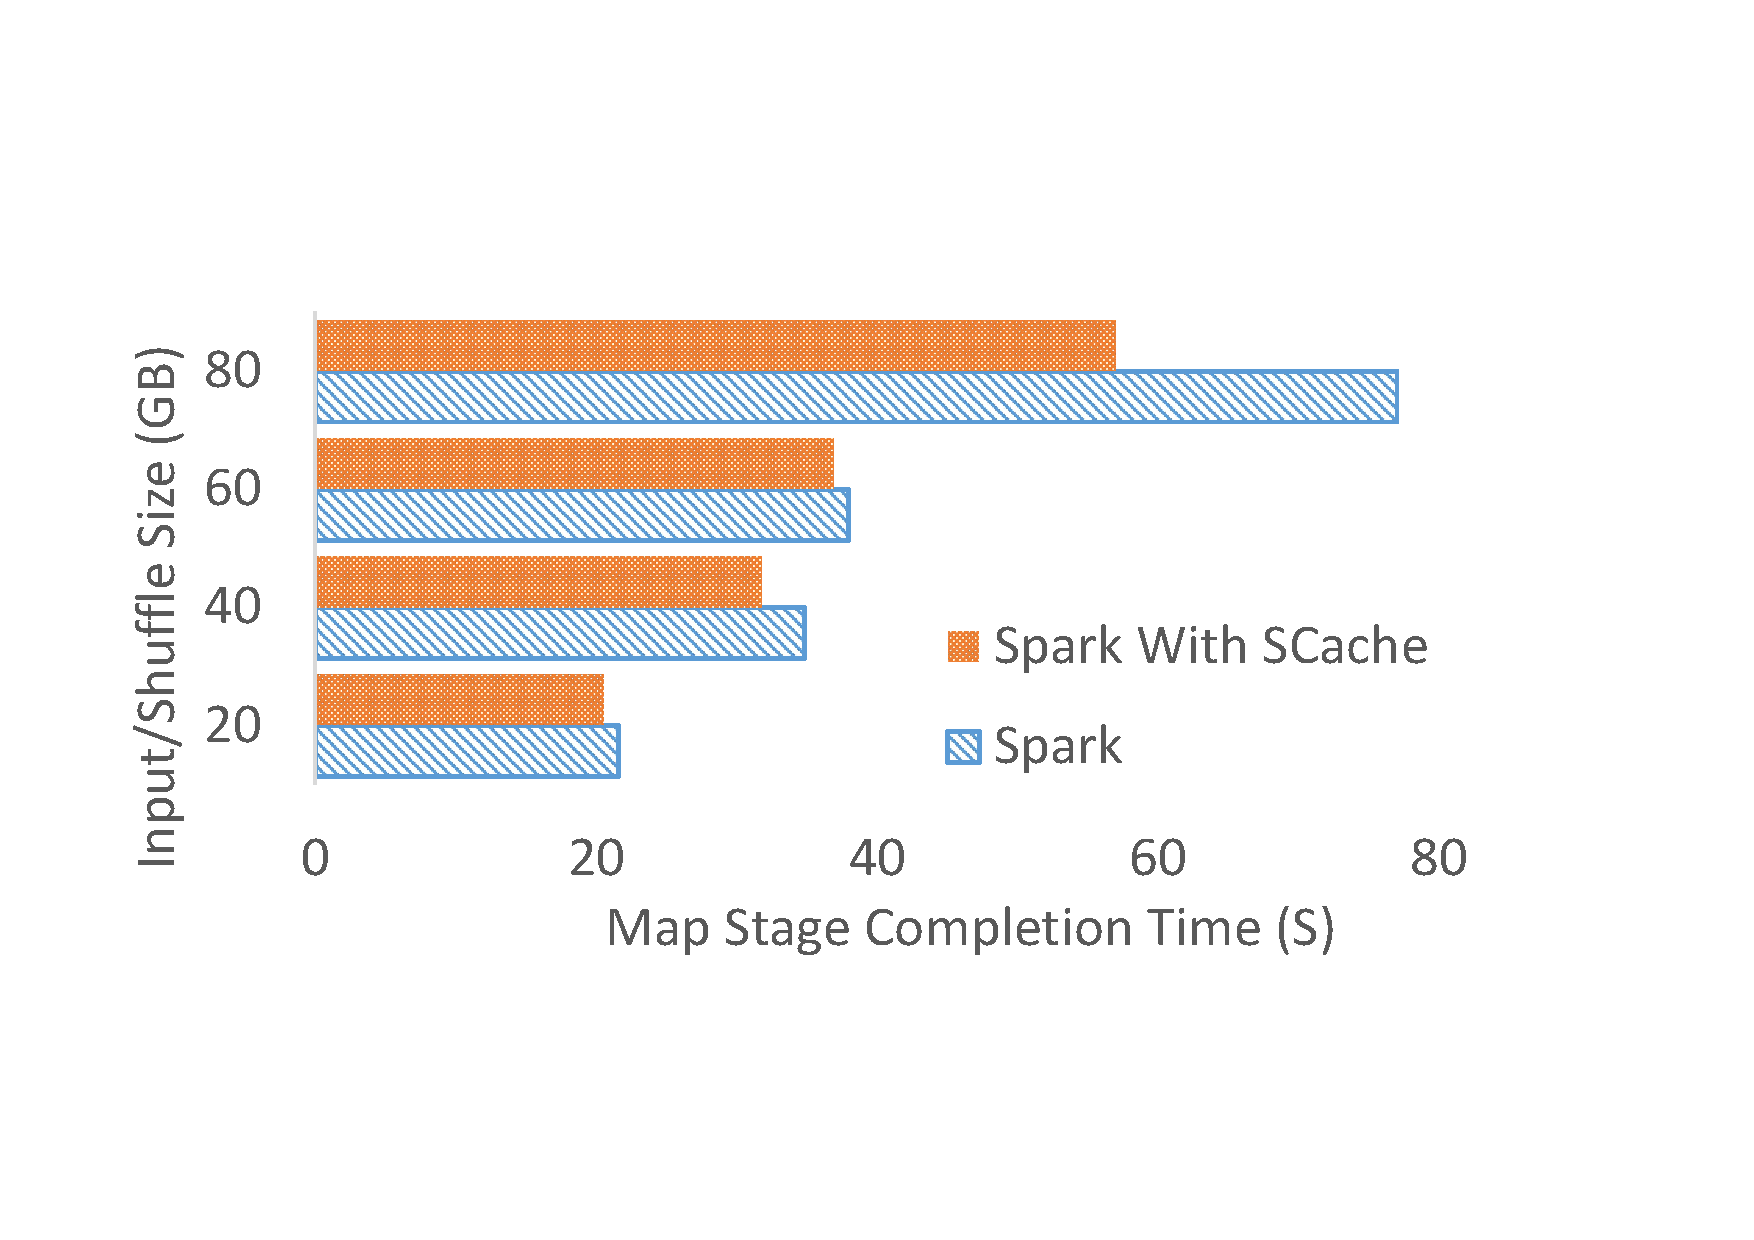
\includegraphics[width=\linewidth]{fig/groupbymapstage}
% 	\caption{Map Stage Completion Time Comparsion}
% 	\label{fig:mapstage}
% \end{subfigure}
% \begin{subfigure}{\linewidth}
% 	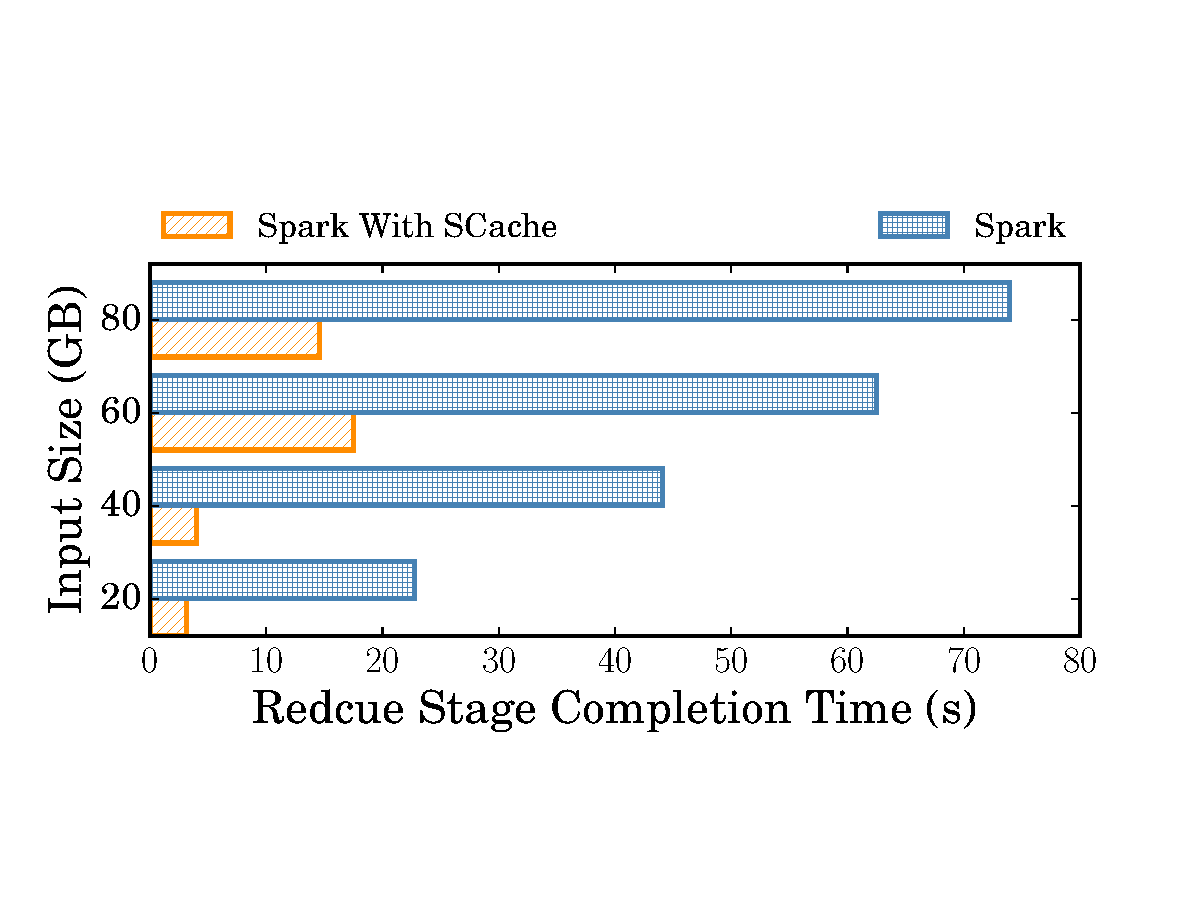
\includegraphics[width=\linewidth]{fig/groupbyreducestage}
% 	\caption{Reduce Stage Completion Time Comparsion}
% 	\label{fig:reducestage}
% \end{subfigure}
% \caption{Stage Completion Time Comparsion of Single Shuffle Test}
% \label{fig:singleshuffle}
% \end{figure}
\subsection{Terasort}
In this part, we evaluate the Terasort \cite{spark-tera}.
Terasort \cite{spark-tera} is a shuffle intensive benchmark for distributed system analysis. It consists of two consecutive shuffles. The first shuffle reads the input data and uses a customized hash partition function for re-partitioning. The second shuffle partitions the data through a range partitioner. As the range bounds set by range partitioner almost match the same pattern of the first shuffle, almost $93\%$ of input data is from one particular map task for each reduce task. It makes the shuffle data transferred through network extremely small under Spark locality preferred task scheduling. So we take the second shuffle as an extreme case to evaluate the scheduling locality for SCache.

As shown in Figure \ref{fig:terasort}, we present the first shuffle as the evaluation of shuffle optimization. At the same time, we use the second the shuffle to evaluate in the dimension of scheduling locality (Figure \ref{fig:terashuffle}). For the first shuffle, Spark with SCache runs 2 $\times$ faster during the reduce stage with the input data in a range from 10GB to 200GB. At the same time, Figure \ref{fig:terashuffle} reveals that SCache pre-scheduling produces exactly same network traffic of second shuffle as Spark, which implies that SCache pre-scheduling can obtain the best locality while balancing the load. In contrast, Spark delays scheduling reduce tasks with the shuffle map output to achieve this optimum.

\subsection{Production Workload}
We also evaluate some shuffle heavy queries from TPC-DS \cite{tpcds}. TPC-DS benchmark is designed for modeling multiple users submitting varied queries (e.g. ad-hoc, interactive OLAP, data mining, etc.). TPC-DS contains 99 queries and is considered as the standardized industry benchmark for testing big data systems. We evaluate the performance of Spark with SCache by picking some of the TPC-DS queries with shuffle intensive attribute. As shown in Figure \ref{fig:tpcds}, on the horizontal axis is query number, and on the vertical axis is query completion time. Spark with SCache outperforms the original Spark in almost all the queries. Furthermore, in many queries, Spark with SCache outperforms original Spark by an order of magnitude. The overall reduction portion of query time that SCache achieved is 40\% on average. Since this evaluation presents the overall job completion time of queries, we believe that our shuffle optimization is promising.
\begin{figure}
	\begin{subfigure}{\linewidth}
		\centering
		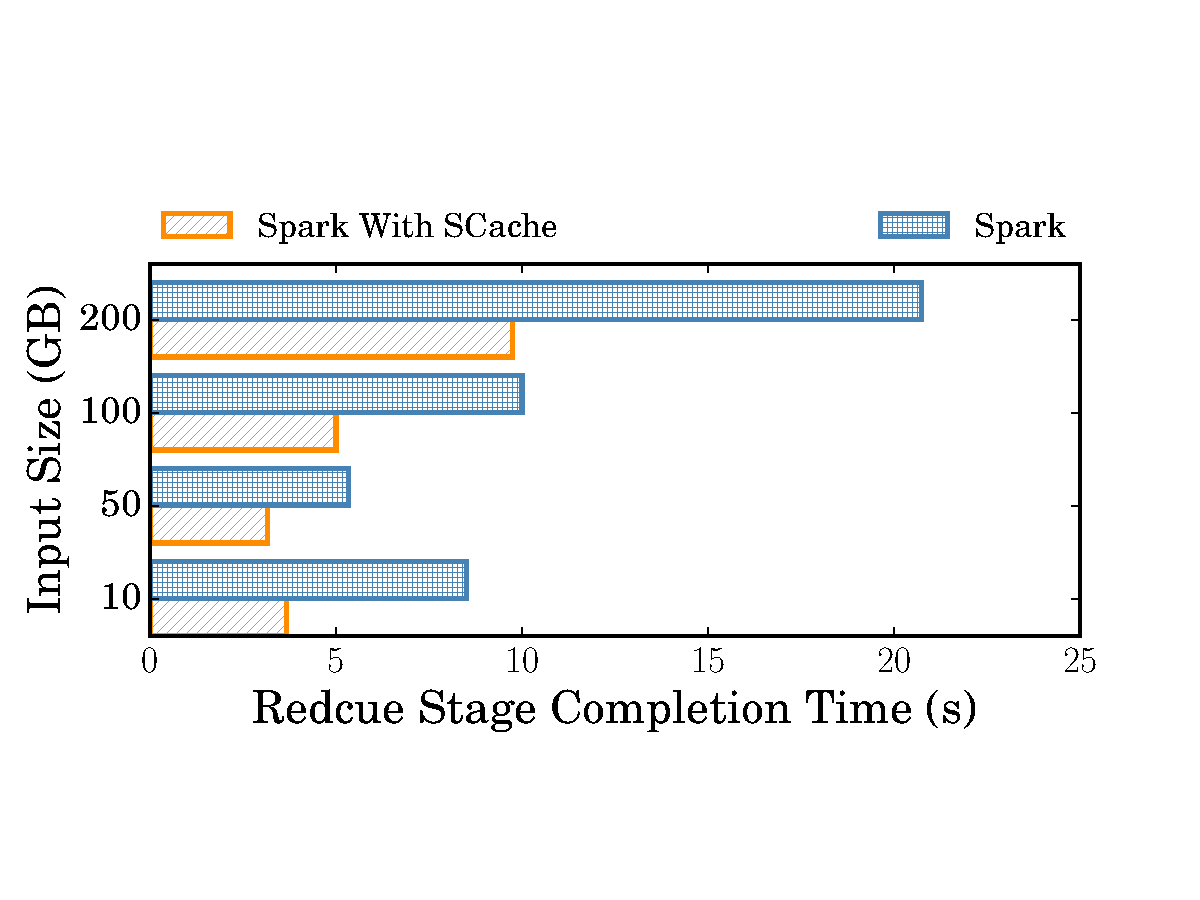
\includegraphics[width=0.915\linewidth]{fig/tera}
		\caption{Reduce Stage Completion Time Comparison of First Shuffle}
		\label{fig:terasort}
	\end{subfigure}
	\vspace{0.08cm}
	\begin{subfigure}{\linewidth}
		\centering
		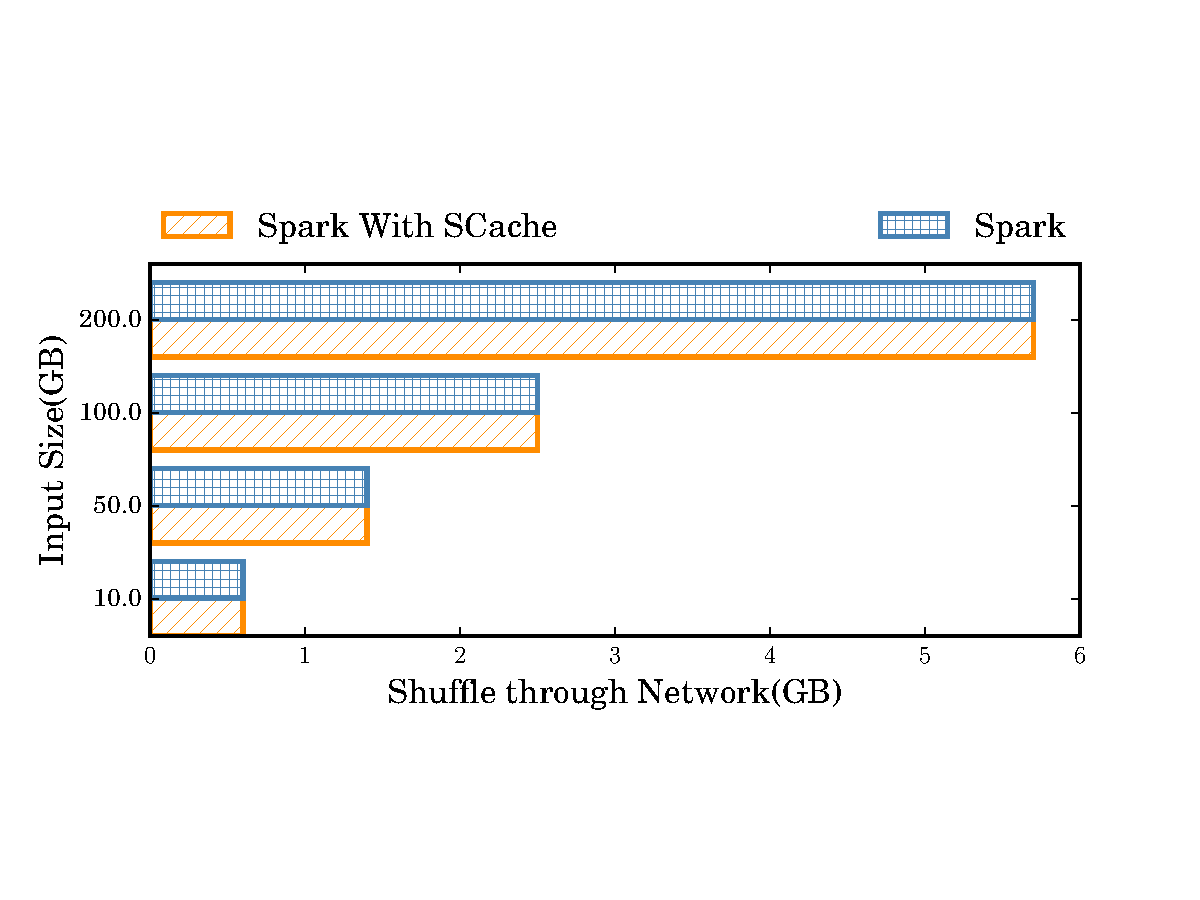
\includegraphics[width=0.915\linewidth]{fig/tera_shuffle}
		\caption{Shuffle Data throuth Network Comparison of Second Shuffle}
		\label{fig:terashuffle}
	\end{subfigure}
	\caption{Terasort Evaluation}
\end{figure}
\subsection{Overhead of Sampling}
In this part, we evaluate the overhead of sampling with different input data sizes on one node and cluster scales. As shown in \ref{fig:sampling}, the overhead of sampling only grows with the increase of input size on each node. But it remains relatively stable when the cluster size scales up. It makes SCache a scalable system in cluster.
\begin{figure*}
	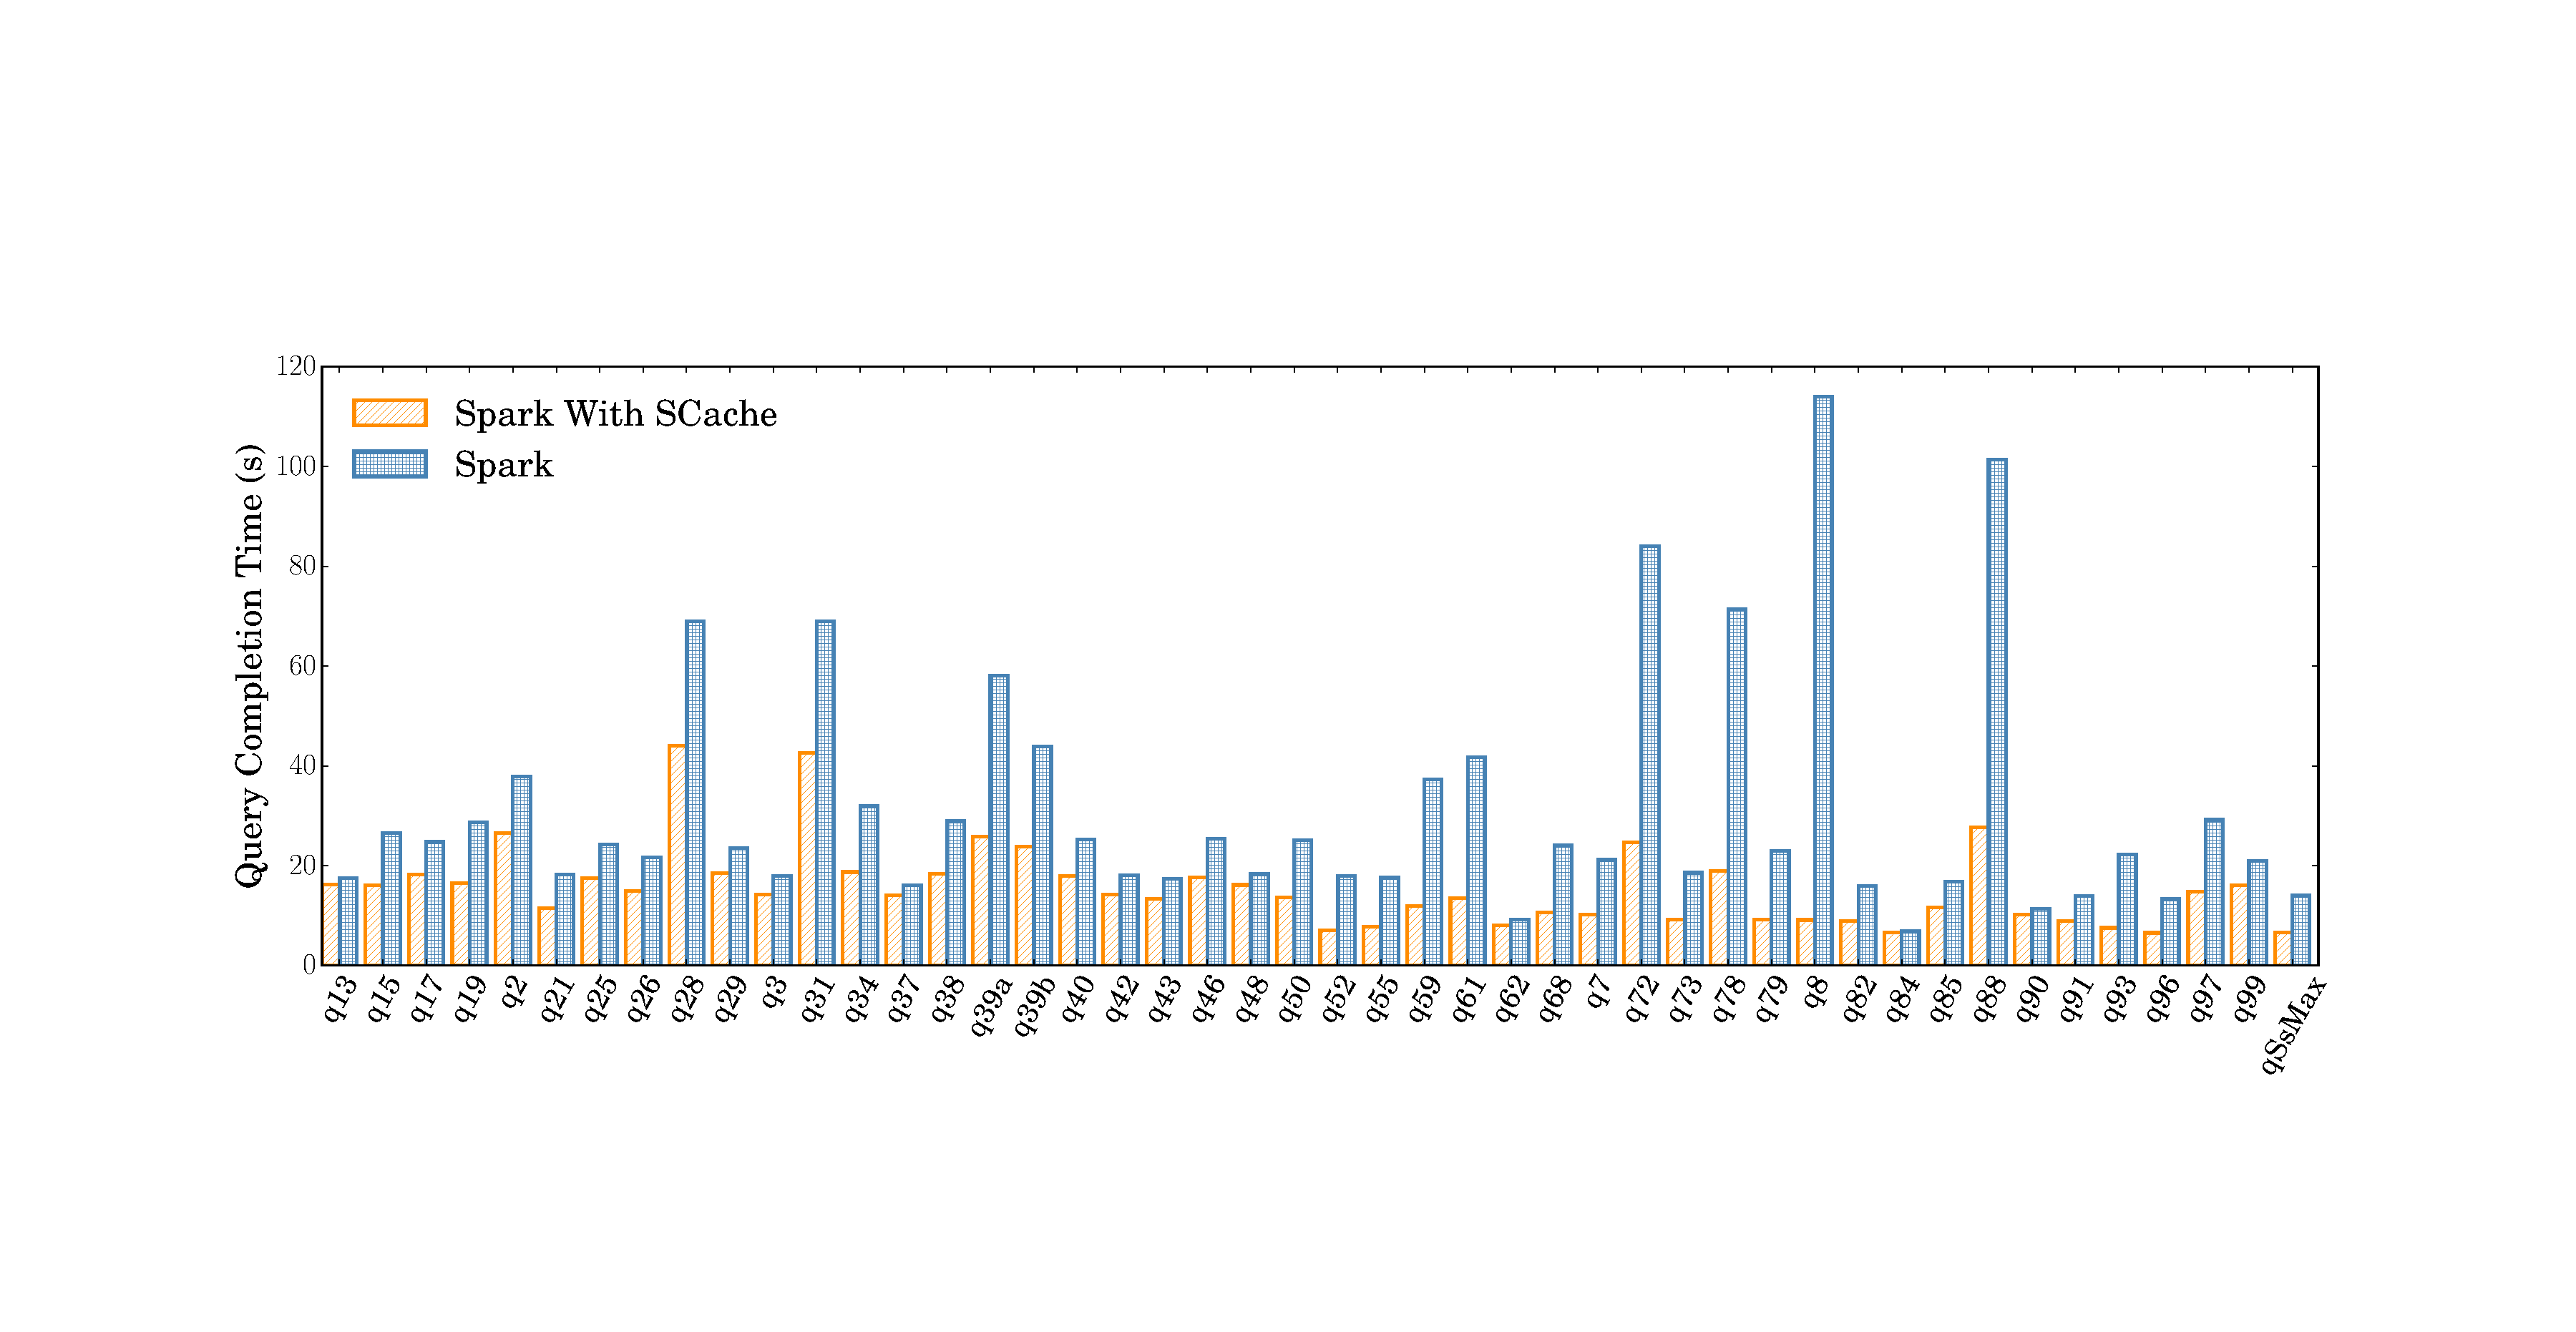
\includegraphics[width=\textwidth]{fig/tpcds}
	\caption{TPC-DS Benchmark Evaluation}
	\label{fig:tpcds}
\end{figure*}


